% !TEX root = DesignDocument.tex


\chapter{Overview, Description and Deliverables}

Within this document is a description of the DoorPanes project. It provides details about the following: clients, the team, preparation needed, requirements, deliverables, implementation and design of components inside the system, the prototypes, testing the prototypes, the results of the tests, sprint progress, schedule of tasks, and the team resumes. It also includes the software contract. This document was created to show the specifications, implementation, and  outline of this project, and most importantly give a guide to individuals working on this project in the future. The goal of this project is to display schedules on office and classroom doors in educational institutions and provide an easier way of communication between the institution and its members or students. 
 

\section{Team Members and Team Name}
The team consists of Andrew Fagrey, Jayson Kjenstad, and Samantha Kranstz. Our team name is the DoorPanes Team.



\section{Clients}
Our clients include Dr. Jeff McGough, Dr. Christer Karlsson, and Brian Butterfield. 

Dr. Jeff McGough is a Professor at South Dakota School of Mines and Technology in Rapid City, SD. He worked on high performance computing at Sun Microsystems, and has been teaching at SDSM\&T for eighteen years. His research focuses on robotics, applied math, and scientific computing.

Dr. Christer Karlsson is an assistant Professor at South Dakota School of Mines and Technology in Rapid City, SD. The former Captain in the Swedish Army has been teaching in the Mathematical and Computer Science department for the last four years. He focuses his research on parallel computing and multi-core architectures. 

Mr. Butterfield co-owns Pixel Pines, a local software business in Rapid City, SD. Brian has spent 17 years in the Telecommunications software industry and became the Technology Manager for a billing and operational support system early in his career. He works closely with South Dakota School of Mines and Technology in Rapid City, SD.

\section{Project}
The objective of this project is to produce a working proof of concept, in other words creating a minimum viable product. The project essentially will be an electronic display on a classroom or faculty office door that has multiple applications communicating with it.   This idea was inspired by Dr. McGough and his constant agony of producing a permanent schedule for his office door. The teacher application will be a responsive web application, with forums or templates to get his or her schedule and messages across to anyone it may concern more easily. The students will have a mobile application\footnote{See Appendix \ref{FutureAppendix}} that will be able to receive push notifications about important messages, such as a class has been canceled or moved to a different room.  The student application will also allow the student to request a reservation of a classroom or a meeting with a professor. The project will be organized and maintained in Microsoft Azure. As for hardware for this project, a tablet will be used; however, this project will not mainly be focused on hardware. The tablet will serve the purpose of displaying our application. 

\subsection{Purpose of the System}
The purpose of this product is to have a more accurate and up to date schedule for faculty members and classrooms. It will inevitably take away the fear of being interrupted, in what appears to be an empty classroom, because the classroom actually has an event or class about to take place in the unoccupied room. It will also provide an immediate update to a office/classroom schedule  if a professor is sick or away on any particular day. 


%\section{Business Need}
%Use this section to define what business need exist and how this software will meet and/or exceed that business need.   


\section{Deliverables}

This project will deliver the following components:

\subsection{Software}

\begin{itemize}
\item Faculty/classroom door tablet application
\item Web API to connect the tablet to the database
\item Faculty responsive web application
\end{itemize}

\subsection{Documentation}
There will be two forms of documentation: external and internal.  This document serves as the external documentation whereas internal documentation will be written within the code. NOTE: Microsoft Visual Studio automatically keeps track of which people authored which parts of the code. 

\section{Business Needs}
Our business model is tiered based on the number of schedules an institute desires to have at a given time. Table \ref{Business Model} estimates possible market pricing for this product. In our business model, the educational institutions will bare the financial burden for our product, while the student app will be free of charge. 
\begin{table}[tbh]
\caption{Business Model. \label{Business Model}}
\begin{center}
\begin{tabular}{|r|l|}
  \hline
  Number of Schedules & Annual Price\\
  \hline
  1-5 & Free \\ \hline
  6-49 & \$1,999 \\
  \hline 
  50-499 & \$4,999 \\
  \hline
  500-999 & \$9,999 \\
  \hline
  1,000-4999 & \$14,999 \\
  \hline
  5,000 + & \$19,999 \\
  \hline
\end{tabular}
\end{center}
\end{table}


\subsection*{Product Description}
Android-based app that allows a professor or office personnel to display a schedule and interact with students. The app is displayed on a device that is mounted onto a door. 
\subsection*{Key Business Goals }
The project goal is to create a proof of concept that could possibly be taken to market with some additional work. 
\subsection*{Primary Market} 
Our primary market for this product is educational institutions.
\subsection*{Assumptions} 
\begin{itemize}
\item Student app will be available on the app stores
\item The institution will permit campus doors to be physically altered.
\item Future work will be done on the project
\item That faculty and student email account have different extensions 
\end{itemize}
\subsection*{Stakeholders}
\begin{itemize}
\item Christer Karlsson
\item Jeff McGough
\item Brian Butterfield
\item Senior design team members
\item Users
\end{itemize} 

\section{System Description}

\subsection{Microsoft Azure}
Azure will play a large role in hosting the Web API, the database, and the responsive web application.

\subsection{Stationary Graphical User Interface}
This electronic component will display schedules and messages on a screen that is mounted to a faculty or classroom door. 

\subsection{Mobile User Interface}
The interface that will enable students to view faculty and classroom schedules, receive notifications, and request classroom reservations.\footnote{See Appendix \ref{FutureAppendix}}

\subsection{Hardware}
Some sort of hardware will be needed to display this product, such as an attachable LCD screen or a touch screen tablet.  

\section{Systems Goals}
Using the components listed above, we will achieve our goal to build and sustain our product. The final product will be able to display faculty and classroom schedules, display notifications, and allow interaction with students via a mobile application.

\section{System Overview and Diagram}
The back end of this program will be developed using Microsoft Azure. This cloud based system will consist of three major components: Microsoft SQL Database, our developed web application, and our API.  All the data for our program will be stored in the database.  The professors and faculty will be able to modify data in this database using our developed web application which is connected to our API.  The cloud system will communicate with our tablet application to display schedules on the doors of the classroom, as well as our mobile application which allows interaction between the student and faculty. See Figure~\ref{systemdiagram} for more information.

\begin{figure}[tbh]
\begin{center}
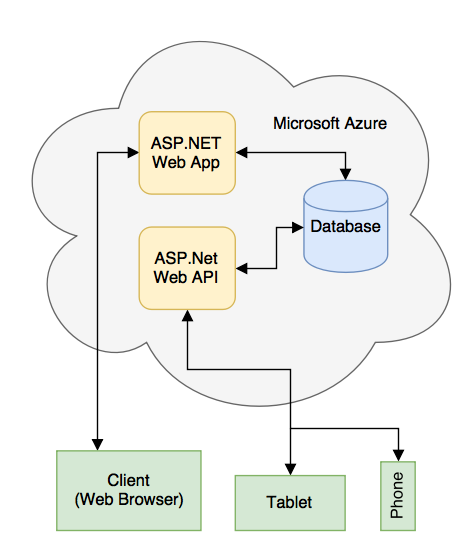
\includegraphics[width=0.65\textwidth]{./DesignImages/OverallDataFlowChp1.png}
\end{center}
\caption{System Diagram \label{systemdiagram}}
\end{figure}

\section{Technologies Overview}
\subsection{System Technology}
\begin{itemize}
\item \href{https://www.visualstudio.com/}{Microsoft Visual Studio} is used for web API, web application, and database code editing.
\item \href{https://azure.microsoft.com/en-us/}{Microsoft Azure} is used for hosting and maintaining the database, web API, and web application.
\item \href{http://square.github.io/retrofit/}{Retrofit} will be the framework used to handle RESTful HTTP requests.
\item \href{https://developer.android.com/studio/index.html}{Android Studio} will be used for the tablet application
\item A \href{http://www.samsung.com/us/mobile/tablets/all-other-tablets/samsung-galaxy-tab-a-8-0-16gb-wi-fi-smoky-titanium-sm-t350nzaaxar/}{Samsung Galaxy Tab} will be used for the tablet hardware.
\end{itemize}

\subsection{Documentation Technology}
\begin{itemize}
\item \LaTeX\ is used to generate this document.
\item \TeX\ maker is an editor used to edit the \LaTeX\ code.
\end{itemize}



%This section should contain a list of specific technologies used to
%develop the system.  The list should contain the name of the
%technology, brief description, link to reference material for further
%understanding, and briefly how/where/why it was used in the %system.
%See Table~\ref{somenumbers}.  This is a floating table environment.


%\begin{table}[tbh]
%\caption{A sample Table ... some numbers. \label{somenumbers}}
%\begin{center}
%\begin{tabular}{|r|l|}
%  \hline
%  7C0 & hexadecimal \\
%  3700 & octal \\ \cline{2-2}
%  11111000000 & binary \\
%  \hline \hline
%  1984 & decimal \\
%  \hline
%\end{tabular}
%\end{center}
%\end{table}

